\begin{figure}[h]
    \centering
    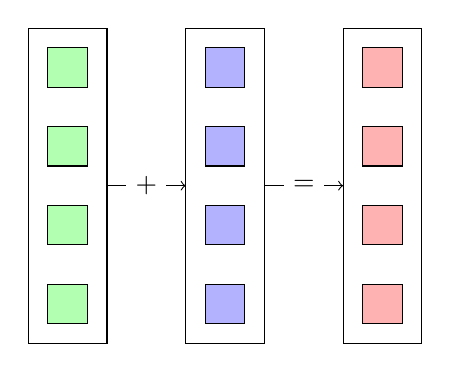
\begin{tikzpicture}

        \foreach \y in {0,..., 3}
            {
                \node[name=1_\y, draw, rectangle, minimum size=0.5cm, fill=green!30] at (0, \y) {};
                \node[name=2_\y, draw, rectangle, minimum size=0.5cm, fill=blue!30] at (2, \y) {};
                \node[name=3_\y, draw, rectangle, minimum size=0.5cm, fill=red!30] at (4, \y) {};
            }
        \draw (-.5, -.5) rectangle (.5, 3.5);
        \draw (1.5, -.5) rectangle (2.5, 3.5);
        \draw (3.5, -.5) rectangle (4.5, 3.5);
        \draw[->] (.5, 1.5) --  node[fill=white] {$+$} (1.5, 1.5);
        \draw[->] (2.5, 1.5) -- node[fill=white] {$=$} (3.5, 1.5);
    \end{tikzpicture}
    \caption{SIMD Processing Example. One instruction is applied to a block of data items.}
    \label{}
\end{figure}